\chapter{Diagramme des cas d'utilisations}


\section{Bibliothèque}
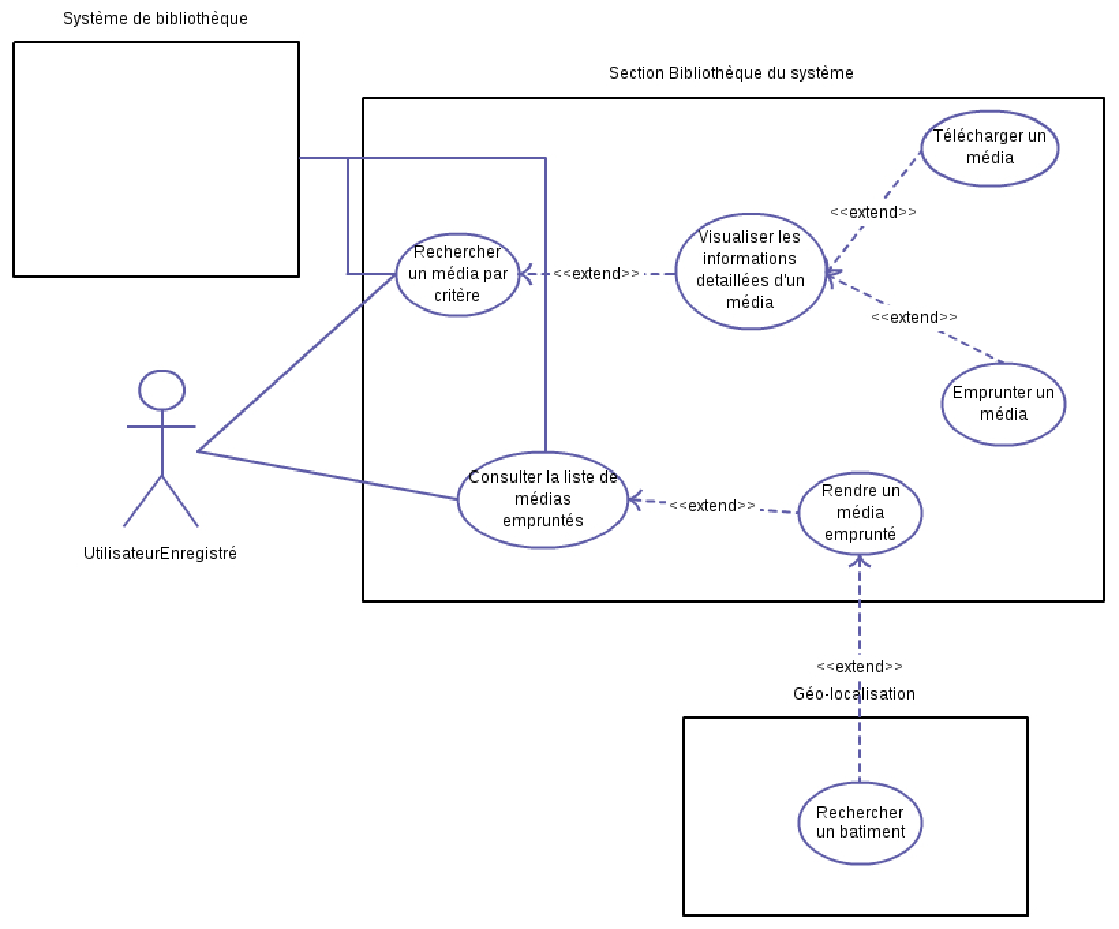
\includegraphics[scale=0.7,angle=90]{cu/Bibliotheque.pdf}
\newpage
\begin{itemize}
\item Rechercher un média par critère: l'utilisateur peut chercher un média selon le titre, l'auteur et le type de média
\item Visualiser les informations détaillées d'un média: l'utilisateur visualise l'auteur, le titre, l'édition, le type de média, le lieu où il se trouve et la disponibilité
\item Télécharger un média: si le média est téchargeable, l'utilisateur peut l'obtenir de cette façon
\item Emprunter un média: sous réserve de ne pas avoir emprunté 5 médias
\item Consulter la liste de médias empruntés: permet de voir les médias non rendu de l'utilisateur
\item Rendre un média emprunté: obligation de retourner le média à la bibliothèque après 2 semaines
\end{itemize}
\newpage


\section{Culturels}
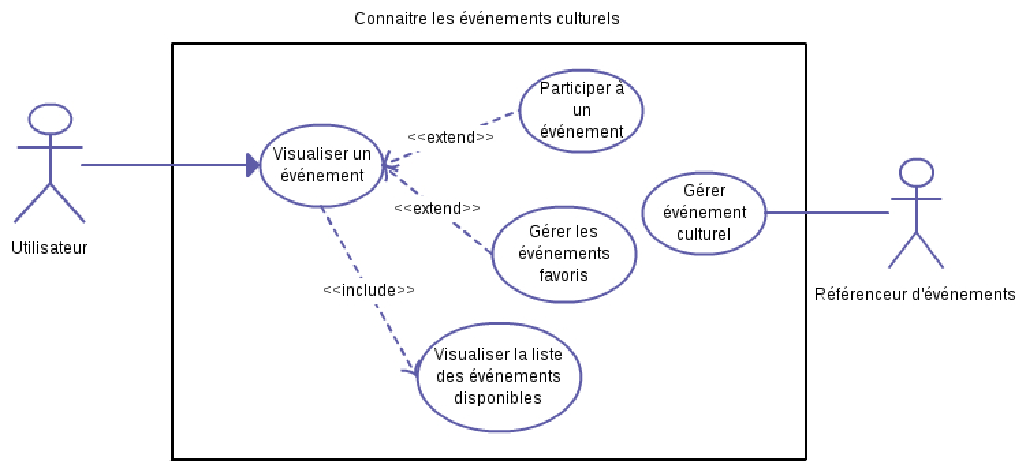
\includegraphics[scale=1,angle=90]{cu/Culturels.pdf}
\newpage
\begin{itemize}
\item Visualiser un événement: effectuer une recherche par critères, puis affiche les informations détaillées de l’événement sélectionné, l’utilisateur peut ajouter l’événement à sa liste de préférences et peut y participer
\item Participer à un événement: l'utilisateur informe qu'il participera à l'événement
\item Gérer les événements favoris: l’utilisateur peut ajouter et enlever des événements de ses favoris
\item Visualiser la liste des événements disponibles: l’affichage se fait selon les préférences, si l’utilisateur n’en a pas, tous les événements de la semaine s’affiche
\item Gérer événement culturel: le référenceur ajoute supprime ou modifie les événements culturels
\end{itemize}
\newpage


\section{Emploi du temps}
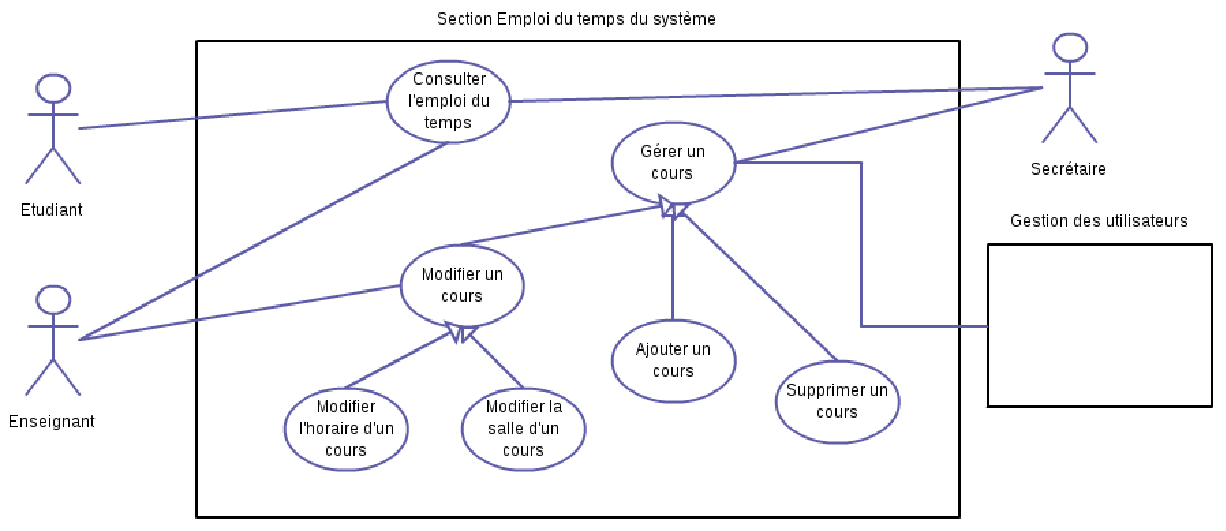
\includegraphics[scale=0.9,angle=90]{cu/EDT.pdf}
\newpage
\begin{itemize}
\item Consulter l‘emploi du temps: permettre aux étudiants et à l’équipe pédagogique d'accéder à la visualisation d’un emploi du temps mis à jour
\item Modifier un cours: modification de l’horaire ou de la salle d’un cours, envoie une notification aux étudiants concernées
\item Modifier l’horaire d’un cours: l’enseignant ou la secrétaire définit le cours à modifier puis la nouvelle horaire, le système gère le choix d’une nouvelle selon les dispositions
\item Modifier la salle d’un cours:  l’enseignant ou la secrétaire définit le cours à modifier puis la nouvelle salle, si elle n’est pas disponible le système propose d’autre salle
\item Gérer un cours: permettre à un utilisateur autorisé de modifier l’emploi du temps qui le concerne, et d’envoyer une notification aux personnes concernées par ces modifications
\item Ajouter un cours: fournir la matière, l’horaire, la salle et le groupe de personnes concernées, si le groupe est déjà occupé un message s’affiche sinon l’emploi du temps est modifié et une notification est envoyé
\item Supprimer un cours: supprimer de l’emploi du temps un cours
\end{itemize}
\newpage


\section{Géo-localisation}
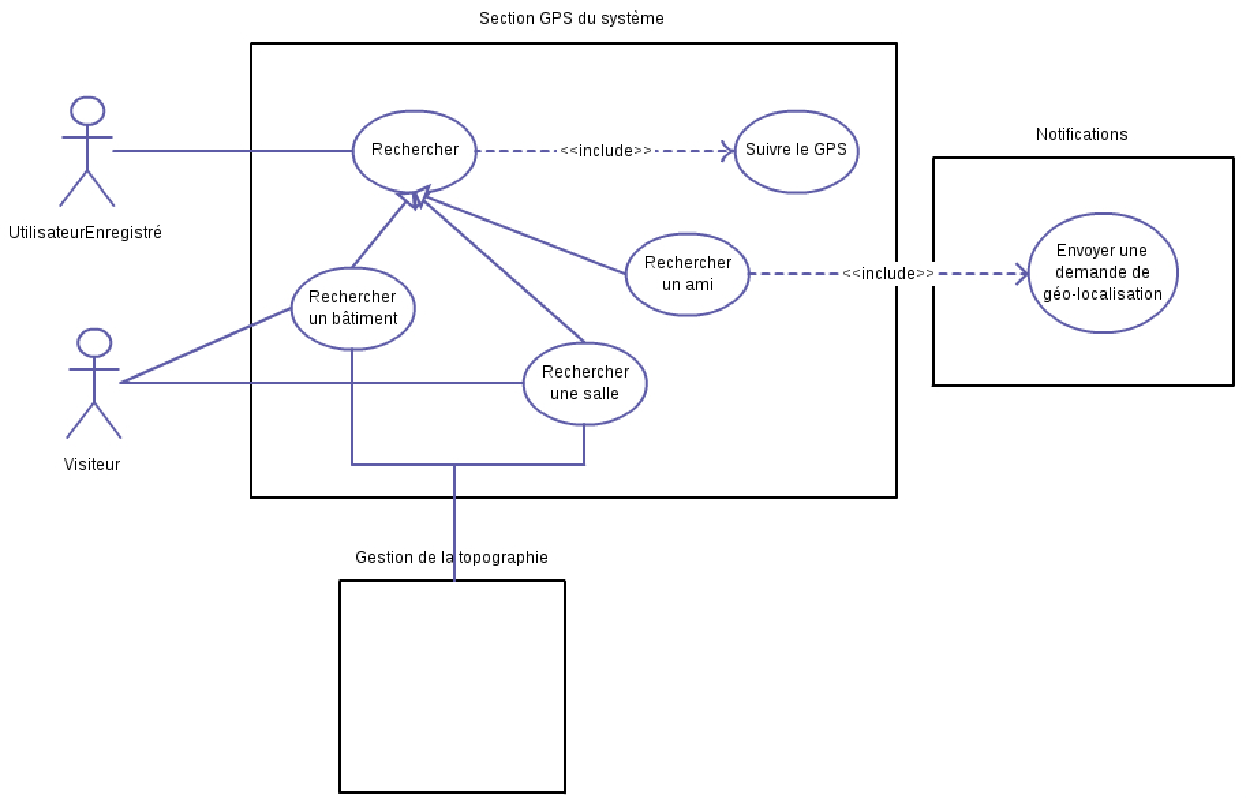
\includegraphics[scale=0.9,angle=90]{cu/GPS.pdf}
\newpage
\begin{itemize}
\item Rechercher: effectue la recherche d’un bâtiment, d’une salle ou d’un ami.
\item Rechercher un ami: effectue une recherche par critère et trace un itinéraire de la position actuelle de l’utilisateur jusque la cible sélectionnée. La géo-localisation d’une personne nécessite l’autorisation de cette dernière via l’envoi d’une notification
\item Rechercher un bâtiment: Recherche l’emplacement d’un bâtiment sur le campus
\item Rechercher une salle: Recherche l’emplacement d’une salle dans un bâtiment
\item Suivre GPS: affichage d’une suite d’instruction permettant de rejoindre un point voulu
\end{itemize}
\newpage


\section{Notifications}
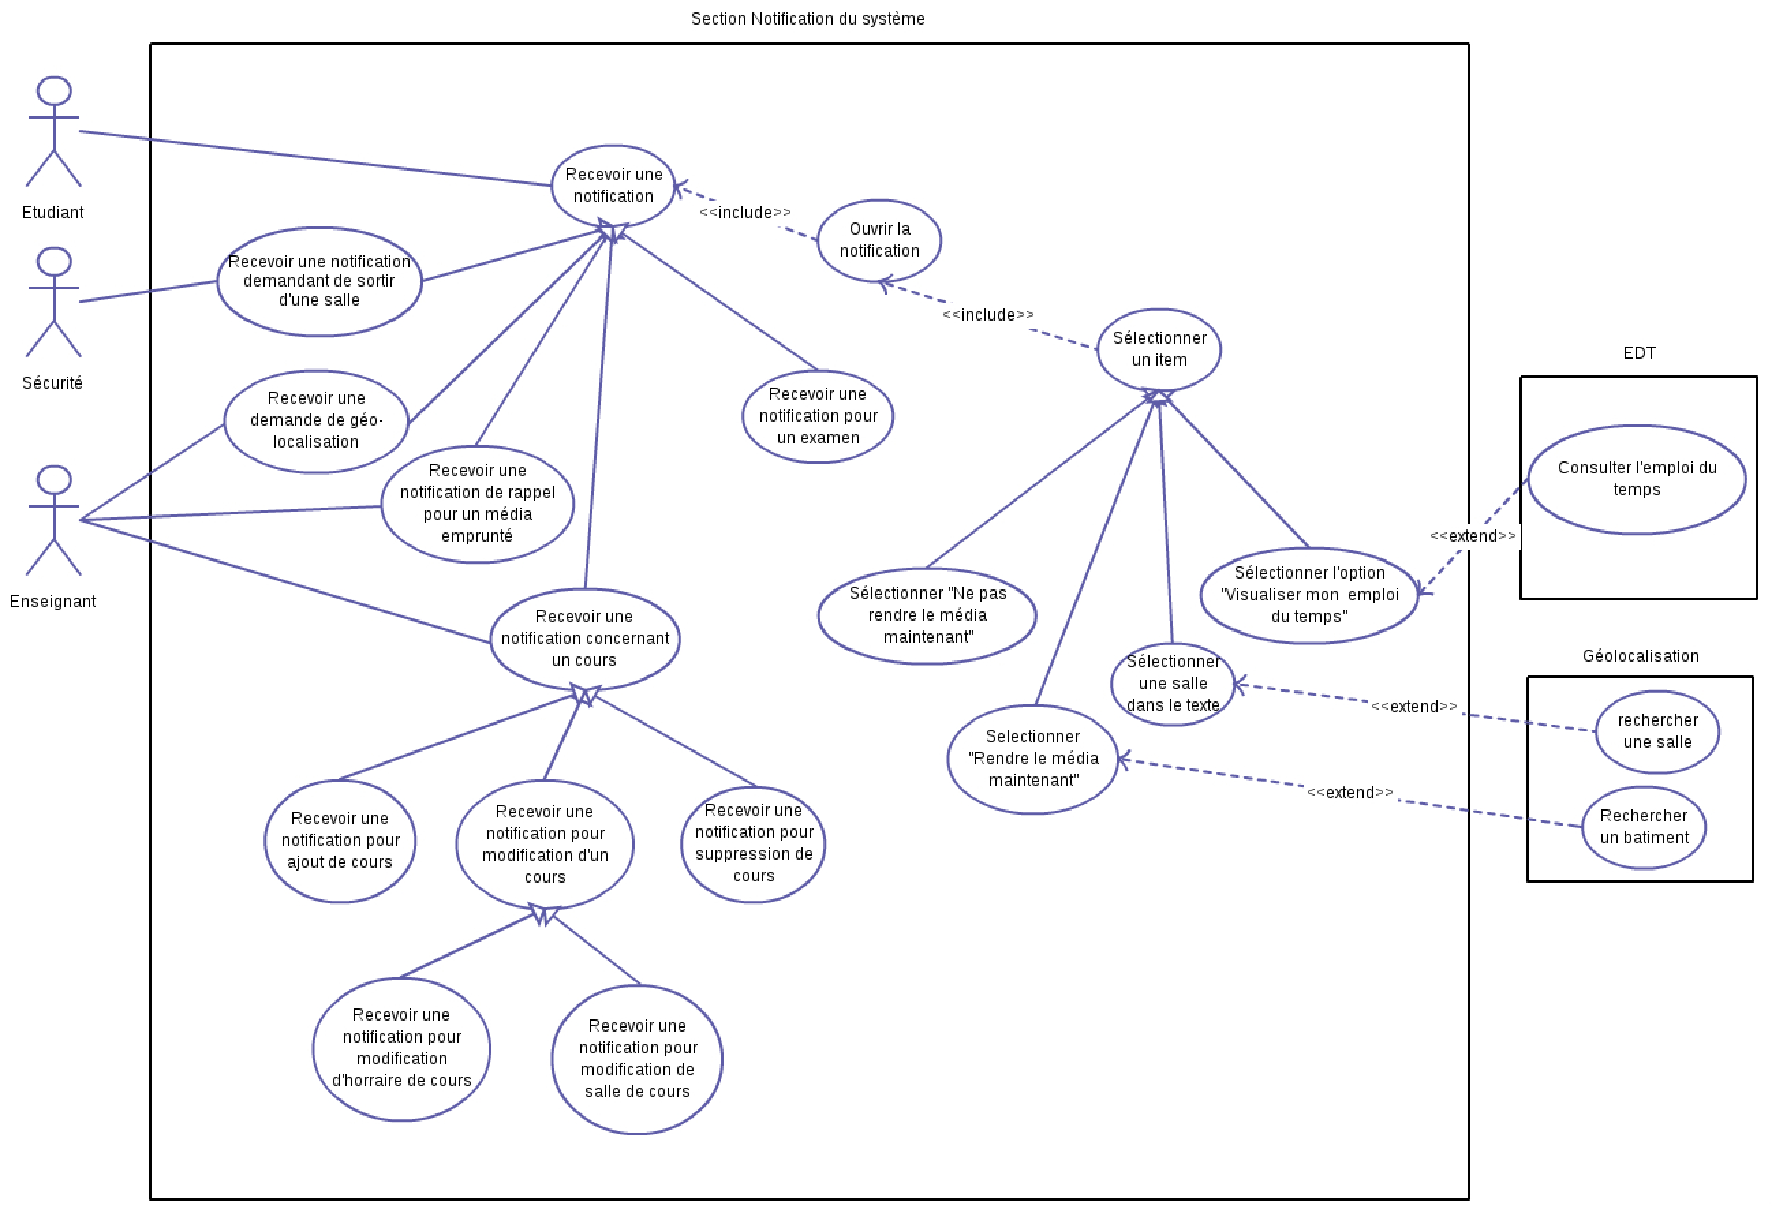
\includegraphics[scale=0.4]{cu/Notifications.pdf}
\begin{itemize}
\item Recevoir une notification: l’utilisateur reçoit une notification affichant différentes informations. Ces informations contiennent des raccourcis vers différentes fonctionnalités du système. La notification peut aussi contenir des requêtes et des liens
\item Recevoir une notification demandant de sortir d'une salle: l'utilisateur est dans un bâtiment après 21 heures. Le système lui envoie une notification pour qu'il sorte
\item Recevoir une demande de géo-localisation:  une connaissance de l'utilisateur le recherche. Il a le choix d'accepter ou non d'être localiser.
\item Recevoir une notification de rappel pour un média emprunté: l'utilisateur doit ramenener un média, il peut être en retard sur la date de rendu. La date est signalé dans la notification
\item Recevoir une notification pour un examen:  l'utilisateur a un examen dans 30 minutes, il reçoit le bâtiment et la salle par notification pour lui rappeler. Il a possibilité de sélectionner le nom du bâtiment pour activer la géo-localisation
\item Ouvrir la notification: l'utilisateur regarde la notification
\item Recevoir une notification concernant un cours: l'utilisateur a soit un cours modifié soit supprimé. Cette notification est envoyé dès qu'une secrétaire ou un professeur le modifie
\item Recevoir une notification pour ajout de cours: l'utilisateur a un cours ajouté, il reçoit dans la notification la date, l'heure, la salle et la matière
\item Recevoir une notification pour modification d'un cours: l'utilisateur a soit un cours déplacé dans un autre salle, soit des horaires changé
\item Recevoir une notification pour suppression de cours: l'utilisateur a un cours supprimé, ce cours peut être ajouté par la suite
\item Recevoir une notification pour modification d'horraire de cours: l'utilisateur reçoit la date, l'heure et la matière du cours concerné et les mêmes informations pour le report
\item Recevoir une notification pour modification de salle de cours: l'utilisateur reçoit la nouvelle salle du cours modifié
\end{itemize}
\newpage


\section{Restauration}
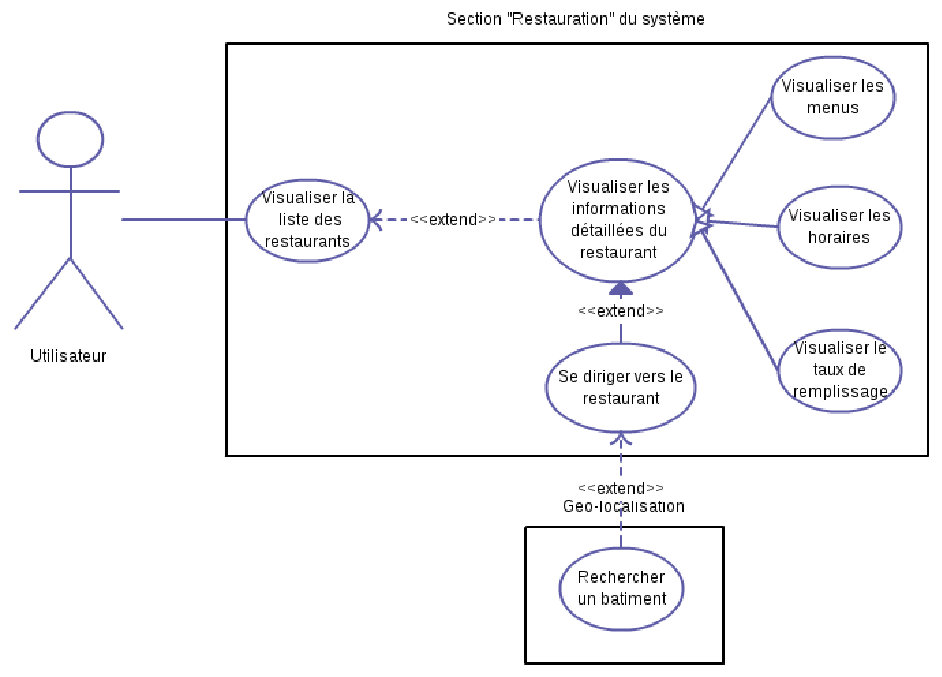
\includegraphics[scale=1,angle=90]{cu/Restauration.pdf}
\newpage
\begin{itemize}
\item Visualiser une liste de restaurants: affiche la liste de restaurants présent sur le campus
\item Visualiser les informations détaillées du restaurant: affiche les informations détaillées du restaurant sélectionné
\item Visualiser les menus: affiche l’ensemble des plats servis
\item Visualiser les horaires: affiche les horaires d’ouverture et de services
\item Visualiser le taux de remplissage: affiche le nombre de personne actuellement présent au restaurant ainsi que sa capacité d’accueil
\item Se diriger vers le restaurant: L’utilisateur déclenche le guidage pour arriver au restaurant choisi
\end{itemize}
\newpage


\section{Sécurité}
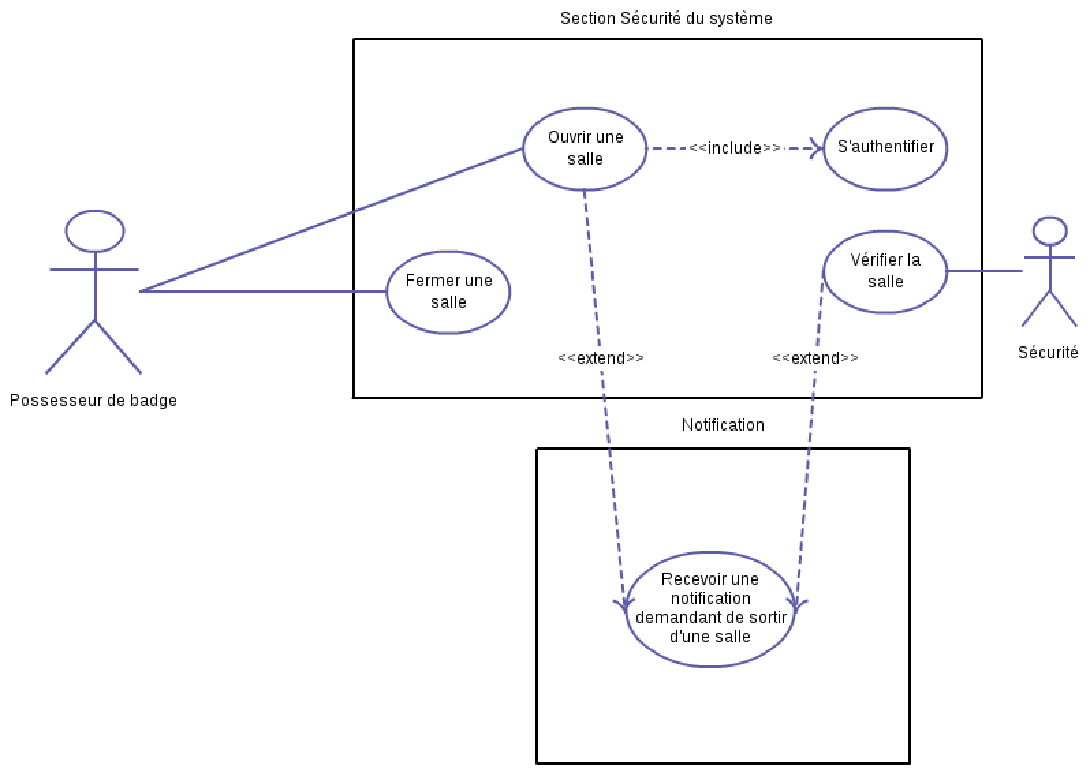
\includegraphics[scale=0.8,angle=90]{cu/Securite.pdf}
\newpage
\begin{itemize}
\item S’authentifier: fournir un login et un mot de passe ou une carte, le système vérifie que le badge a un niveau d’utilisation suffisant
\item Ouvrir une salle: le possesseur de badge est devant la salle, il doit s’authentifier
\item Fermer une salle: seul un possesseur de badge peut fermer la salle, il doit passer son badge pour pouvoir la fermer
\item Vérifier une salle: le système(les capteurs) vérifie la présence ou non de personne dans la salle au moment de la fermeture automatique
\end{itemize}
